% Provenance (never printed): see sources/outline_sources.md (Year 2: fractional
% crystallisation, Bowen's series, compatible and incompatible elements, mixing and
% assimilation, layered intrusions).
% Curves from figdata/bachelor-2/differentiation.py (Bowen 1913 plagioclase loop, Rayleigh and
% equilibrium laws, Wilcox 1954 Paricutin analyses and mass balance, AFC closed form,
% Tegner et al. 2023 Skaergaard whole-rock data); exercise and problem values in the Book 4
% scratch calculator calc/ch08.py.
\chapter{Magmatische differentiatie}\label{ch:b2:magmatic-differentiation}

Op 20 februari 1943 begon in het westen van Mexico een vulkaan uit te barsten, en dat
duurde negen jaar. Zijn eerste lava's waren basaltische andesieten met \qty{55}{\percent}
silica; zijn laatste, in februari 1952, waren andesieten met iets meer dan
\qty{60}{\percent}. De vulkaan, Parícutin, schakelde intussen niet over op een andere bron,
en zijn lava's werden een voor een geanalyseerd naarmate ze naar buiten kwamen. Het
\omterm{def:b2:magma-emplacement:magma}{magma} eronder veranderde zelf: het liet kristallen groeien en achter, en het verteerde
een deel van het granitische gesteente eromheen. Een \omterm{def:b2:magma-emplacement:magma}{magma} dat de mantel als basalt verlaat, kan
als rhyoliet eindigen, en de gesteenten die het onderweg achterlaat, leggen vast hoe dat ging.
Dit hoofdstuk volgt een \omterm{def:b2:magma-emplacement:magma}{magma} terwijl het afkoelt: de volgorde waarin mineralen kristalliseren,
de wetten die zeggen hoe hoofd- en \omterm{def:b2:elements-in-the-earth:trace}{sporenelementen} veranderen wanneer kristallen worden verwijderd,
de gesteenten die uit die kristallen worden opgebouwd, en wat er gebeurt wanneer het \omterm{def:b2:magma-emplacement:magma}{magma} een
ander \omterm{def:b2:magma-emplacement:magma}{magma} of de korst opneemt.
% ledger: wilcox54:paricutin

\begin{recall}
\textbf{Uit Boek~2}: stollingsgesteenten en hun texturen; de volgorde
waarin mineralen uit een basaltisch \omterm{def:b2:magma-emplacement:magma}{magma} kristalliseren, olivijn eerst en kwarts als laatste,
gevonden met de experimenten van Bowen. \textbf{Uit het scheikundeboek van het tweede jaar universiteit}:
binaire fasediagrammen, vaste oplossingen en de hefboomregel. \textbf{Uit
Boek~3}: plagioklaas, een vaste oplossing tussen anorthiet \ce{CaAl2Si2O8} en albiet
\ce{NaAlSi3O8}, en de andere gesteentevormende silicaten; slijpplaatjes tussen gekruiste
nicols. \textbf{Uit \cref{ch:b2:elements-in-the-earth}}: de verdelingscoëfficiënten mineraal--smelt
en de globale, $\bar D = \sum_i x_i D_i$, compatibele en \omterm{def:b2:elements-in-the-earth:partition}{incompatibele
elementen}, genormaliseerde diagrammen en de \omterm{prop:b2:elements-in-the-earth:normalised}{europiumanomalie}. \textbf{Uit
\cref{ch:b2:isotope-geochemistry}}: isotopenverhoudingen als tracers en de
\omterm{prop:b2:isotope-geochemistry:mixing}{menghyperbool}. \textbf{Uit \cref{ch:b2:mantle-melting}}: het eutecticum diopsied--anorthiet,
\omterm{def:b2:mantle-melting:peritectic}{incongruent smelten}, ternaire diagrammen en \omterm{def:b2:mantle-melting:primary}{primaire magma's}.
\end{recall}

\section{Kristallisatiereeksen}\label{sec:b2:magmatic-differentiation:sequences}

Een basaltisch \omterm{def:b2:magma-emplacement:magma}{magma} kristalliseert niet al zijn mineralen tegelijk. Bowen vond
experimenteel dat olivijn normaal als eerste kristalliseert, tussen 1200 en
\qty{1300}{\celsius}; dat het calciumrijke plagioklaas ongeveer begint waar pyroxeen
begint; en dat de laatste, silicarijke vloeistof kaliveldspaat, kwarts en
eventueel muscoviet geeft, rond 750 tot \qty{800}{\celsius}. Daartussen stapelen de mafische
mineralen zich niet eenvoudig op: elk reageert met de vloeistof tot het volgende.
% ledger: earle:bowen (Book 2), tulane:bowen (Book 2)

\begin{definition}[Reactiereeks van Bowen]\label{def:b2:magmatic-differentiation:bowen}
De \emph{reactiereeks van Bowen}\index{reactiereeks van Bowen} is de volgorde waarin
de gewone silicaten uit een afkoelend basaltisch \omterm{def:b2:magma-emplacement:magma}{magma} kristalliseren, als twee takken
die aan het eind samenkomen. In de \emph{discontinue tak} reageert elk mafisch mineraal
met de vloeistof tot een nieuw mineraal met een andere structuur: olivijn,
pyroxeen, amfibool, biotiet. In de \emph{continue tak} kristalliseert plagioklaas
de hele weg door, terwijl zijn samenstelling continu verandert van calciumrijk
naar natriumrijk. De laatste vloeistof kristalliseert kaliveldspaat, muscoviet en
kwarts.
\end{definition}
% ledger: earle:bowen (Book 2)

\begin{omfigure}
\centering
\begin{tikzpicture}[font=\small, x=1cm, y=1cm,
  mn/.style={draw, rounded corners=2pt, fill=white, inner sep=3pt, minimum width=2.3cm,
             align=center}]
\draw[-{Stealth[length=4pt]}, thick, gray] (-1.3,0.3) -- (-1.3,-6.0);
\node[rotate=90, anchor=south, font=\scriptsize, gray] at (-1.4,-2.85) {dalende temperatuur};
\node[anchor=east, font=\scriptsize] at (-1.5,0) {$\approx$ 1200--\qty{1300}{\celsius}};
\node[anchor=east, font=\scriptsize] at (-1.5,-5.6) {$\approx$ 750--\qty{800}{\celsius}};
\node[mn] (ol) at (1,0) {olivijn};
\node[mn] (px) at (1,-1.4) {pyroxeen};
\node[mn] (am) at (1,-2.8) {amfibool};
\node[mn] (bt) at (1,-4.2) {biotiet};
\draw[-{Stealth[length=4pt]}, thick] (ol) -- (px);
\draw[-{Stealth[length=4pt]}, thick] (px) -- (am);
\draw[-{Stealth[length=4pt]}, thick] (am) -- (bt);
\node[font=\scriptsize, align=center] at (1,0.8) {discontinue tak\\(bij elke stap een nieuw mineraal)};
\node[mn] (ca) at (6,-1.4) {calciumrijk\\plagioklaas};
\node[mn] (na) at (6,-4.2) {natriumrijk\\plagioklaas};
\fill[left color=white, right color=white, top color=orange!35, bottom color=orange!8]
  (5.75,-2.0) rectangle (6.25,-3.6);
\draw[-{Stealth[length=4pt]}, thick] (ca) -- (na);
\node[font=\scriptsize, align=center] at (6,0.8) {continue tak\\(één mineraal, veranderende samenstelling)};
\node[mn, minimum width=7.2cm] (last) at (3.5,-5.6) {kaliveldspaat, muscoviet, kwarts};
\draw[-{Stealth[length=4pt]}, thick] (bt) -- (bt|-last.north);
\draw[-{Stealth[length=4pt]}, thick] (na) -- (na|-last.north);
\end{tikzpicture}
\par\smallskip{\small De \omterm{def:b2:magmatic-differentiation:bowen}{reactiereeks van Bowen}. Olivijn en calciumrijk plagioklaas
kristalliseren als eerste uit een basaltisch \omterm{def:b2:magma-emplacement:magma}{magma}; links reageert elk mafisch mineraal met
de vloeistof tot het volgende, rechts wordt het plagioklaas steeds rijker aan
natrium; de laatste, silicarijke vloeistof geeft kaliveldspaat, muscoviet en kwarts.
De temperaturen zijn typische waarden voor basaltisch \omterm{def:b2:magma-emplacement:magma}{magma} bij lage druk.}
\end{omfigure}
% ledger: earle:bowen (Book 2)

De twee takken komen overeen met de twee soorten fasediagram van
\cref{ch:b2:mantle-melting}. Een discontinue reactie is het \omterm{def:b2:mantle-melting:peritectic}{incongruente smelten} van
enstatiet in omgekeerde richting: forsterietkristallen reageren met een silicarijkere vloeistof
tot enstatiet. De continue tak is een vaste oplossing. Bowen mat haar in 1913
aan synthetische plagioklazen: hij hield elke samenstelling op een bekende temperatuur en
zocht naar glas en kristallen. Anorthiet smelt bij \qty{1550}{\celsius}, albiet bij
ongeveer \qty{1100}{\celsius}, en elk tussenliggend plagioklaas smelt over een interval
tussen een onderste kromme, de solidus, en een bovenste, de liquidus (de figuur
hieronder).
% ledger: bowen13:plagioclase, bowen14:mgo-sio2

\begin{omfigure}
\centering
\begin{tikzpicture}
\begin{axis}[omrecord, width=0.78\linewidth, height=6.4cm,
  xmin=0, xmax=100, ymin=1050, ymax=1600,
  xlabel={anorthiet (\unit{\percent}, moleculair)}, ylabel={temperatuur (\unit{\celsius})},
  y tick label style={/pgf/number format/1000 sep={}}, unbounded coords=discard,
  tick label style={font=\scriptsize}, label style={font=\small}]
\addplot[very thick, black] table[x=an, y=T_liq] {figdata/out/bachelor-2-differentiation-plag-curve.dat};
\addplot[very thick, black, dashed] table[x=an, y=T_sol] {figdata/out/bachelor-2-differentiation-plag-curve.dat};
\addplot[only marks, mark=*, mark size=1.5pt, blue!70!black] table[x=an, y=T_liq] {figdata/out/bachelor-2-differentiation-plag-data.dat};
\addplot[only marks, mark=o, mark size=1.7pt, blue!70!black] table[x=an, y=T_sol] {figdata/out/bachelor-2-differentiation-plag-data.dat};
\draw[densely dotted, red!70!black, thick] (axis cs:50,1560) -- (axis cs:50,1287);
\draw[red!70!black, thick] (axis cs:50,1450) -- (axis cs:80.6,1450);
\draw[red!70!black, thick] (axis cs:33.3,1394) -- (axis cs:70.6,1394);
\draw[red!70!black, thick] (axis cs:13.9,1287) -- (axis cs:50,1287);
\addplot[only marks, mark=*, mark size=1.4pt, red!70!black] coordinates {(50,1450) (80.6,1450) (33.3,1394) (70.6,1394) (13.9,1287) (50,1287)};
\node[font=\scriptsize] at (axis cs:30,1530) {vloeistof};
\node[font=\scriptsize, align=center] at (axis cs:83,1200) {plagioklaas\\(vaste oplossing)};
\node[font=\scriptsize, anchor=west] at (axis cs:2,1430) {liquidus (doorgetrokken lijn)};
\node[font=\scriptsize, anchor=west] at (axis cs:42,1160) {solidus (gestreept)};
\node[font=\scriptsize, anchor=south, red!70!black, fill=white, inner sep=1pt] at (axis cs:68,1452) {\qty{1450}{\celsius}};
\node[font=\scriptsize, anchor=north, red!70!black, fill=white, inner sep=1pt] at (axis cs:31,1284) {\qty{1287}{\celsius}};
\end{axis}
\end{tikzpicture}
\par\smallskip{\small De plagioklaasveldspaten bij atmosferische druk, uit de
afschrikexperimenten van Bowen (1913): begin (cirkels) en einde (stippen) van het
smelten, met krommen door de metingen getrokken. In rood de \omterm{def:b2:magmatic-differentiation:crystallisation}{evenwichtskristallisatie}
van een vloeistof met \qty{50}{\percent} anorthiet: het eerste kristal, bij
\qty{1450}{\celsius}, heeft \qty{81}{\percent} anorthiet; bij \qty{1394}{\celsius}
bestaan kristallen met \qty{71}{\percent} naast een vloeistof met \qty{33}{\percent}; de laatste
vloeistof, bij \qty{1287}{\celsius}, heeft \qty{14}{\percent} (\cref{exo:b2:magmatic-differentiation:1}).}
\end{omfigure}
% ledger: bowen13:plagioclase

Een vloeistof die een vaste oplossing kristalliseert, verrijkt zich in de component die
bij de laagste temperatuur smelt: het eerste plagioklaas uit een vloeistof met
\qty{50}{\percent} anorthiet heeft er \qty{81}{\percent}, en de vloeistof schuift op naar
albiet. Wat daarna gebeurt, hangt ervan af of de kristallen met de vloeistof blijven
uitwisselen.

\begin{definition}[Evenwichtskristallisatie en fractionele kristallisatie]
\label{def:b2:magmatic-differentiation:crystallisation}
Bij \emph{evenwichtskristallisatie}\index{evenwichtskristallisatie} blijven de
kristallen tot het einde in chemisch evenwicht met de hele vloeistof, en stellen ze
zich opnieuw in naarmate de vloeistof verandert; het systeem eindigt met de samenstelling
waarmee het begon. Bij \emph{fractionele kristallisatie}\index{fractionele kristallisatie}
wordt elk kristal, eenmaal gevormd, aan de reactie met de
vloeistof onttrokken, doordat het uitzakt, tegen de wanden van de kamer wordt geplakt, of
door latere groei wordt afgeschermd; de vloeistof ontwikkelt zich dan alsof de kristallen
uit het systeem waren gehaald.
\end{definition}

Bij \omterm{def:b2:magmatic-differentiation:crystallisation}{evenwichtskristallisatie} verandert het plagioklaas van de figuur hierboven van
\qty{81}{\percent} naar \qty{50}{\percent} anorthiet terwijl het groeit, waarbij elk kristal
zich door diffusie opnieuw met de vloeistof in evenwicht stelt, en de laatste vloeistof verdwijnt bij
de solidus, \qty{1287}{\celsius}. Diffusie in veldspaat is traag, en natuurlijke
kristallen houden zelden bij: het binnenste van elk kristal raakt van de vloeistof afgesneden,
die zich dan gedraagt als bij \omterm{def:b2:magmatic-differentiation:crystallisation}{fractionele kristallisatie} en kan doorgaan tot samenstellingen
dicht bij albiet. De figuur in de laatste paragraaf van dit hoofdstuk berekent beide paden.
% ledger: bowen13:plagioclase

\begin{definition}[Afdalingslijn van de vloeistof]\label{def:b2:magmatic-differentiation:lld}
De \emph{afdalingslijn van de vloeistof}\index{afdalingslijn van de vloeistof} van een \omterm{def:b2:magma-emplacement:magma}{magma} is de
opeenvolging van samenstellingen die zijn vloeistof aanneemt terwijl het kristalliseert, uitgezet in een
variatiediagram of een fasediagram.
\end{definition}

Een \omterm{def:b2:magmatic-differentiation:lld}{afdalingslijn van de vloeistof} is een eigenschap van de vloeistof alleen. Lava's die met
kristallen erin uitvloeien, liggen er niet precies op, en Wilcox gebruikte bij zijn studie van de lava's van
Parícutin zowel hun analyses van het totale gesteente als de samenstellingen van hun
grondmassa, het vloeibare deel, berekend door de kristallen eraf te trekken.
% ledger: wilcox54:groundmass

\section{Fractionele kristallisatie van de hoofdelementen}\label{sec:b2:magmatic-differentiation:majors}

Kristallen verwijderen verandert de samenstelling van de vloeistof op een eenvoudige, lineaire manier,
en het oudste hulpmiddel om dat te lezen is een grafiek van elk oxide tegen silica.

\begin{definition}[Harkerdiagram]\label{def:b2:magmatic-differentiation:harker}
Een \emph{Harkerdiagram}\index{Harkerdiagram} (silicavariatiediagram) zet het
massapercentage van elk oxide van een reeks verwante gesteenten uit tegen hun
massapercentage \ce{SiO2}, één paneel per oxide.
\end{definition}


De lava's van Parícutin vertonen zulke trends (de \omterm{def:b2:magmatic-differentiation:harker}{Harkerdiagrammen} na de volgende
propositie): naarmate silica stijgt, dalen magnesia, kalk en aluinaarde en stijgt kali. Dat is
wat het verwijderen van olivijn en plagioklaas zou doen:
olivijn neemt magnesia en ijzer weg, plagioklaas kalk en aluinaarde, en beide laten
de vloeistof rijker aan silica en alkaliën achter. Of het verwijderen van bekende mineralen de
trends kwantitatief kan verklaren, is een vraag van massabalans.

\begin{proposition}[Massabalans van het verwijderen van kristallen]\label{prop:b2:magmatic-differentiation:lever}
Laat een oudermagma met samenstelling $\mathbf p$ (een vector van massafracties van oxiden)
mineralen met samenstellingen $\mathbf m_1, \dots, \mathbf m_k$ kristalliseren in massa's
$x_1, \dots, x_k$ per massa-eenheid ouder, en zij $\mathbf d$ de samenstelling
van de overgebleven vloeistof. Dan geldt
\[
\mathbf p = \Big(1 - \sum_i x_i\Big)\mathbf d + \sum_i x_i \mathbf m_i .
\]
Bij één mineraal ligt de ouder op het rechte lijnstuk tussen de vloeistof en het
mineraal in elk variatiediagram, en de verwijderde massafractie is
$x = (p_j - d_j)/(m_j - d_j)$ voor elk oxide $j$: de hefboomregel.
\end{proposition}

\begin{proof}
Elk oxide blijft behouden: de massa $p_j$ van oxide $j$ in een massa-eenheid ouder komt
terecht in de vloeistof, met massa $1 - \sum_i x_i$ en concentratie $d_j$, of in de
mineralen. Dit voor elke $j$ uitschrijven geeft de vectorvergelijking. Met één mineraal
luidt ze $\mathbf p = (1-x)\mathbf d + x\mathbf m$, een punt van het lijnstuk van
$\mathbf d$ naar $\mathbf m$ dat het verdeelt in de verhouding $x : (1-x)$, in elk paar
assen; één component oplossen geeft $x$.
\end{proof}

\begin{omfigure}
\centering
\begin{tikzpicture}
\begin{groupplot}[group style={group size=2 by 2, horizontal sep=1.6cm, vertical sep=1.3cm},
  width=0.44\linewidth, height=4.3cm, omrecord, xmin=54.5, xmax=60.8,
  tick label style={font=\scriptsize}, label style={font=\small},
  xtick={55,56,57,58,59,60}]
\nextgroupplot[ylabel={\ce{MgO} (\unit{\percent})}, ymin=3.2, ymax=6.0]
\addplot[only marks, mark=*, mark size=1.3pt, blue!70!black] table[x=SiO2, y=MgO] {figdata/out/bachelor-2-differentiation-paricutin.dat};
\nextgroupplot[ylabel={\ce{CaO} (\unit{\percent})}, ymin=6.0, ymax=7.6]
\addplot[only marks, mark=*, mark size=1.3pt, blue!70!black] table[x=SiO2, y=CaO] {figdata/out/bachelor-2-differentiation-paricutin.dat};
\nextgroupplot[ylabel={\ce{K2O} (\unit{\percent})}, ymin=0.7, ymax=1.9, xlabel={\ce{SiO2} (\unit{\percent})}]
\addplot[only marks, mark=*, mark size=1.3pt, blue!70!black] table[x=SiO2, y=K2O] {figdata/out/bachelor-2-differentiation-paricutin.dat};
\node[font=\scriptsize, anchor=west] at (axis cs:55.1,0.80) {1943};
\node[font=\scriptsize, anchor=east] at (axis cs:60.0,1.82) {1952};
\nextgroupplot[ylabel={\ce{Al2O3} (\unit{\percent})}, ymin=17.0, ymax=19.0, xlabel={\ce{SiO2} (\unit{\percent})}]
\addplot[only marks, mark=*, mark size=1.3pt, blue!70!black] table[x=SiO2, y=Al2O3] {figdata/out/bachelor-2-differentiation-paricutin.dat};
\end{groupplot}
\end{tikzpicture}
\par\smallskip{\small \omterm{def:b2:magmatic-differentiation:harker}{Harkerdiagrammen} van de 22 lava's van Parícutin die
Wilcox (1954) analyseerde, uitgevloeid van februari 1943 (laagste silica) tot februari 1952. Terwijl
silica met vijf procent stijgt, dalen magnesia, kalk en aluinaarde en verdubbelt kali
bijna.}
\end{omfigure}
% ledger: wilcox54:table2, wilcox54:paricutin

Met meerdere mineralen vindt men de massa's door de behoudsvergelijkingen van
evenveel oxiden op te lossen. Wilcox deed dat in 1954 grafisch; tegenwoordig is het een klein lineair
stelsel.

\begin{method}[Massabalans met kleinste kwadraten]\label{met:b2:magmatic-differentiation:massbalance}
Om te toetsen of een dochtervloeistof $\mathbf d$ uit een ouder $\mathbf p$ ontstaat door
het verwijderen van mineralen $\mathbf m_1, \dots, \mathbf m_k$ (en zo nodig het toevoegen van een
geassimileerd gesteente, ingevoerd met een negatieve massa): (1) schrijf voor elk oxide $j$ het
behoud van de propositie herschikt als een lineaire vergelijking in de massa's die
per \qty{100}{g} ouder worden verwijderd,
\[
\sum_i x_i\,(m_{ij} - d_j) = 100\,(p_j - d_j);
\]
(2) los met precies $k$ oxiden, gekozen uit die welke de mineralen het sterkst veranderen, het
$k \times k$-stelsel op; los het met meer oxiden op met kleinste kwadraten (minimaliseer de som
van de gekwadrateerde verschillen tussen beide leden); (3) bereken de dochter opnieuw uit
de gevonden massa's en vergelijk haar oxide per oxide met de analyse: residuen groter
dan de analysefouten, of een negatieve massa voor een mineraal, verwerpen het model.
\end{method}

Wilcox koos silica, aluinaarde en magnesia als zijn drie controle-oxiden, en drie
materialen: olivijn met samenstelling Fo$_{80}$, plagioklaas An$_{70}$, en het gemiddelde
van vier granitische xenolieten (\qty{72.5}{\percent} \ce{SiO2}, \qty{3.6}{\percent}
\ce{K2O}) die in de lava's werden gevonden. Hij toonde aan dat geen combinatie van alleen olivijn en
plagioklaas de reeks verklaart, en dat het toevoegen van \qty{25.4}{g} xenoliet en het
verwijderen van \qty{2.9}{g} olivijn en \qty{9.6}{g} plagioklaas uit
\qty{100}{g} grondmassa van de eerste lava \qty{112.9}{g} materiaal oplevert dat
dicht bij de grondmassa van de lava van 1950 ligt. Zijn drie vergelijkingen exact oplossen
geeft \qty{24.6}{g}, \qty{3.1}{g} en \qty{9.9}{g}; kleinste kwadraten over zeven oxiden
geeft een ander antwoord, \qty{28.7}{g}, \qty{2.4}{g} en \qty{5.7}{g}, een herinnering
dat zulke resultaten van de gekozen controle-oxiden afhangen. Hoe dan ook nam het \omterm{def:b2:magma-emplacement:magma}{magma} meer
graniet op dan het kristalliseerde. De lava's van Parícutin leggen een open systeem vast, het
onderwerp van de laatste paragraaf.
% ledger: wilcox54:mass-balance, wilcox54:xenoliths, wilcox54:groundmass

\section{Sporenelementen}\label{sec:b2:magmatic-differentiation:trace}

Een \omterm{def:b2:elements-in-the-earth:trace}{sporenelement} verandert de mineralen die kristalliseren niet; het volgt ze,
met zijn globale verdelingscoëfficiënt $\bar D$ (\cref{ch:b2:elements-in-the-earth}),
hier $D$ geschreven, tussen de kristallen die op elk moment ontstaan en de vloeistof.

\begin{theorem}[Fractioneringswet van Rayleigh]\label{thm:b2:magmatic-differentiation:rayleigh}
Bij volmaakte \omterm{def:b2:magmatic-differentiation:crystallisation}{fractionele kristallisatie} met een constante globale verdelingscoëfficiënt
$D$ is de concentratie van een \omterm{def:b2:elements-in-the-earth:trace}{sporenelement} in de vloeistof
\[
\frac{C_L}{C_0} = F^{\,D-1},
\]
waarin $C_0$ zijn concentratie in de oorspronkelijke vloeistof is en $F$ de massafractie
overgebleven vloeistof. Dit is de
\emph{fractioneringswet van Rayleigh}\index{fractioneringswet van Rayleigh}.
\end{theorem}

\begin{proof}
Zij $M$ de massa vloeistof. Wanneer een kleine massa $-\mathrm dM > 0$ kristallen
ontstaat, alleen op dat moment in evenwicht met de vloeistof, voert ze het element mee in de
concentratie $DC_L$. De massa van het element in de vloeistof, $MC_L$, verandert dus
met $\mathrm d(MC_L) = DC_L\,\mathrm dM$. Uitgewerkt geeft dat $M\,\mathrm dC_L = (D-1)C_L\,
\mathrm dM$, dus $\mathrm dC_L/C_L = (D-1)\,\mathrm dM/M$. Integreren vanaf $M_0$,
waar $C_L = C_0$, geeft $\ln(C_L/C_0) = (D-1)\ln(M/M_0)$, en $F = M/M_0$.
\end{proof}

\begin{proposition}[Evenwichtskristallisatie van een sporenelement]
\label{prop:b2:magmatic-differentiation:equilibrium}
Als de kristallen met de vloeistof in evenwicht blijven, geldt $C_L/C_0 = 1/(D + F(1-D))$.
\end{proposition}

\begin{proof}
De hele kristalmassa $1-F$ (per eenheid beginmassa) bevat $DC_L$, dus het
massabehoud van het element luidt $C_0 = FC_L + (1-F)DC_L$.
\end{proof}

\begin{corollary}[Verhoudingen van incompatibele elementen]\label{cor:b2:magmatic-differentiation:ratio}
Voor twee elementen met verdelingscoëfficiënten $D_1$ en $D_2$ verandert de verhouding van hun
concentraties in de vloeistof bij \omterm{def:b2:magmatic-differentiation:crystallisation}{fractionele kristallisatie} met de factor $F^{\,D_1-D_2}$.
Zijn beide sterk incompatibel ($D_1, D_2 \ll 1$), dan verandert de verhouding
nauwelijks: ze behoudt de waarde van het oudermagma, en dus van zijn bron.
\end{corollary}

\begin{proof}
Deel de twee wetten van Rayleigh op elkaar: $(C_1/C_2)/(C_{1,0}/C_{2,0}) = F^{D_1-1}/F^{D_2-1}$;
voor $F = 0.5$ en $D_1 - D_2 = 0.05$ is de factor $0.5^{0.05} = 0.97$.
\end{proof}

\begin{omfigure}
\centering
\begin{tikzpicture}
\begin{axis}[omrecord, width=0.78\linewidth, height=6.4cm, ymode=log,
  xmin=0, xmax=1, ymin=0.01, ymax=100, x dir=reverse,
  xlabel={overgebleven fractie vloeistof $F$}, ylabel={$C_L/C_0$},
  legend columns=3, legend style={font=\scriptsize, at={(0.02,0.97)}, anchor=north west},
  tick label style={font=\scriptsize}, label style={font=\small}]
\addplot[thick, red!75!black] table[x=F, y=d0.01] {figdata/out/bachelor-2-differentiation-rayleigh.dat};
\addlegendentry{$D = 0.01$}
\addplot[thick, orange!80!black] table[x=F, y=d0.1] {figdata/out/bachelor-2-differentiation-rayleigh.dat};
\addlegendentry{0.1}
\addplot[thick, olive] table[x=F, y=d0.5] {figdata/out/bachelor-2-differentiation-rayleigh.dat};
\addlegendentry{0.5}
\addplot[thick, teal] table[x=F, y=d2] {figdata/out/bachelor-2-differentiation-rayleigh.dat};
\addlegendentry{2}
\addplot[thick, blue!70!black] table[x=F, y=d5] {figdata/out/bachelor-2-differentiation-rayleigh.dat};
\addlegendentry{5}
\addplot[thick, violet] table[x=F, y=d10] {figdata/out/bachelor-2-differentiation-rayleigh.dat};
\addlegendentry{10}
\addplot[thick, dashed, forget plot, red!75!black] table[x=F, y=e0.01] {figdata/out/bachelor-2-differentiation-rayleigh.dat};
\addplot[thick, dashed, forget plot, orange!80!black] table[x=F, y=e0.1] {figdata/out/bachelor-2-differentiation-rayleigh.dat};
\addplot[thick, dashed, forget plot, teal] table[x=F, y=e2] {figdata/out/bachelor-2-differentiation-rayleigh.dat};
\addplot[thick, dashed, forget plot, violet] table[x=F, y=e10] {figdata/out/bachelor-2-differentiation-rayleigh.dat};
\end{axis}
\end{tikzpicture}
\par\smallskip{\small Concentratie van een \omterm{def:b2:elements-in-the-earth:trace}{sporenelement} in de vloeistof tegen de
overgebleven fractie vloeistof, voor globale verdelingscoëfficiënten van 0.01 tot 10:
\omterm{def:b2:magmatic-differentiation:crystallisation}{fractionele kristallisatie} (doorgetrokken, wet van Rayleigh) en \omterm{def:b2:magmatic-differentiation:crystallisation}{evenwichtskristallisatie}
(gestreept, voor $D = 0.01$, 0.1, 2 en 10). \omterm{def:b2:elements-in-the-earth:partition}{Incompatibele elementen} stijgen hoogstens met $1/F$;
\omterm{def:b2:elements-in-the-earth:partition}{compatibele elementen} kelderen, des te sneller naarmate $D$ groot is, en \omterm{def:b2:magmatic-differentiation:crystallisation}{fractionele
kristallisatie} haalt ze er bijna volledig uit.}
\end{omfigure}

De figuur hierboven laat zich in twee richtingen lezen. \omterm{def:b2:elements-in-the-earth:partition}{Incompatibele elementen} ($D \ll 1$) gedragen zich
vrijwel gelijk: hun concentratie stijgt bijna als $1/F$, zodat een vloeistof die
tienvoudig in zirkonium is verrijkt, ongeveer negen tiende van haar massa heeft gekristalliseerd. \omterm{def:b2:elements-in-the-earth:partition}{Compatibele
elementen} zijn veel gevoeliger. Nikkel gaat in olivijn met een verdelingscoëfficiënt
van ongeveer 5 in hete, magnesiumrijke vloeistoffen: gemeten op 3.8 bij
\qty{1550}{\celsius} en 5.0 bij \qty{1400}{\celsius}, stijgt hij met ongeveer 0.8 per
\qty{100}{\celsius} afkoeling; strontium gaat in
plagioklaas met ongeveer 2.7; een basalt die een vijfde van zijn massa als
olivijn kristalliseert, verliest meer dan de helft van zijn nikkel (\cref{exo:b2:magmatic-differentiation:5}). Nikkel is daarom het
gevoeligste archief van olivijnfractionering, en een nikkelrijke basalt ligt
dicht bij een \omterm{def:b2:mantle-melting:primary}{primair magma} (\cref{ch:b2:mantle-melting}).
% ledger: matzen12:dni, white07:kd-basalt

Twee opmerkingen bakenen de reikwijdte van deze wetten af. Ten eerste is $D$ geen constante: hij verandert
wanneer een nieuw mineraal zich bij de kristalliserende associatie voegt, en de wet wordt dan
in etappes toegepast (\cref{exo:b2:magmatic-differentiation:12}). Ten tweede beschrijven dezelfde vergelijkingen, met de rollen van vaste stof en
vloeistof verwisseld, het smelten van een bron; hoe batch- en fractioneel
smelten de \omterm{def:b2:elements-in-the-earth:trace}{sporenelementen} fractioneren, komt aan bod in Boek~5.

\section{Cumulaten en gelaagde intrusies}\label{sec:b2:magmatic-differentiation:cumulates}

Waar gaan de kristallen heen die uit een \omterm{def:b2:magma-emplacement:magma}{magma} worden verwijderd? In een magmakamer die
langzaam afkoelt, zakken ze naar de bodem, groeien ze aan de wanden en het dak, en bouwen ze gesteenten van
een bijzondere soort op.

\begin{definition}[Cumulaat; gelaagde intrusie]\label{def:b2:magmatic-differentiation:cumulate}
Een \emph{cumulaat}\index{cumulaat} is een stollingsgesteente gevormd door de ophoping van
kristallen (de cumuluskristallen) uit een \omterm{def:b2:magma-emplacement:magma}{magma}, samen met de mineralen die later zijn gegroeid
uit de vloeistof die ertussen gevangen zat (het intercumulusmateriaal); zijn samenstelling
is die van kristallen plus een beetje vloeistof, niet die van enig \omterm{def:b2:magma-emplacement:magma}{magma}. Een
\emph{gelaagde intrusie}\index{gelaagde intrusie} is een groot, langzaam afgekoeld lichaam van mafische of
ultramafische cumulaten in lagen, dat de \omterm{def:b2:magmatic-differentiation:crystallisation}{fractionele kristallisatie} vastlegt van
het \omterm{def:b2:magma-emplacement:magma}{magma} dat het vulde.
\end{definition}

De Skaergaard-intrusie in Oost-Groenland, ongeveer \qty{56}{Ma} oud, is de
referentie. Haar gelaagde gabbro's dagzomen over zo'n 11 bij \qty{8}{km}, en leggen de
ononderbroken differentiatie van een tholeïtische basalt vast: een Gelaagde Serie groeide op de
bodem, Randseries aan de wanden en het dak, en de twee kwamen samen in de Sandwichhorizont,
waar de laatste, meest geëvolueerde vloeistof in het binnenste kristalliseerde (de figuur hieronder).
De bodemcumulaten worden van onder naar boven verdeeld in een Verborgen Zone, die niet dagzoomt,
en de dagzomende Onderste, Middelste en Bovenste Zone. Haar
onderzoekers schatten de massafractie $F$ vloeistof die over was toen elk niveau kristalliseerde, gefit
langs het referentieprofiel van de Gelaagde Serie met
\[
F = \num{1.091e-7}\,H^2 - \num{5.9064e-4}\,H + 0.7678
\]
($H$ in meter boven de basis van de Onderste Zone). Een kwart van het \omterm{def:b2:magma-emplacement:magma}{magma} was al
gekristalliseerd, in de wanden, het dak en een verborgen zone, toen de dagzomende
bodemopeenvolging begon; de Sandwichhorizont, $F = 0$, ligt zo'n \qty{2.2}{km} hoger
(\cref{exo:b2:magmatic-differentiation:7}).
% ledger: tegner23:skaergaard

\begin{omfigure}
\centering
\begin{tikzpicture}[x=1cm, y=1cm, font=\scriptsize]
\fill[gray!20] (-5.4,-0.5) rectangle (5.4,4.9);
\node[anchor=south west] at (-5.35,4.35) {nevengesteente};
\fill[orange!35] (-4.6,0) rectangle (4.6,1.1);
\fill[orange!22] (-4.2,1.1) rectangle (4.2,1.9);
\fill[orange!12] (-3.8,1.9) rectangle (3.8,2.55);
\fill[blue!12] (-4.6,4.3) rectangle (4.6,3.75);
\fill[blue!20] (-4.2,3.75) rectangle (4.2,3.25);
\fill[blue!28] (-3.8,3.25) rectangle (3.8,2.85);
\fill[orange!35] (-4.6,1.1) rectangle (-4.2,3.75);
\fill[orange!35] (4.2,1.1) rectangle (4.6,3.75);
\fill[orange!22] (-4.2,1.9) rectangle (-3.8,3.25);
\fill[orange!22] (3.8,1.9) rectangle (4.2,3.25);
\fill[red!40] (-3.8,2.55) rectangle (3.8,2.85);
\draw[thick] (-4.6,0) rectangle (4.6,4.3);
\draw (-4.2,1.1) rectangle (4.2,3.75);
\draw (-3.8,1.9) rectangle (3.8,3.25);
\foreach \y in {0.2,0.4,0.6,0.8,1.3,1.5,1.7,2.1,2.3} \draw[gray] (-3.0,\y) -- (3.0,\y);
\node[fill=orange!35, inner sep=1.5pt] at (0,0.5) {Onderste Zone};
\node[fill=orange!22, inner sep=1.5pt] at (0,1.5) {Middelste Zone};
\node[fill=orange!12, inner sep=1.5pt] at (0,2.2) {Bovenste Zone};
\node[font=\scriptsize\bfseries] at (0,2.7) {Sandwichhorizont};
\node at (0,4.02) {Bovenste Randserie};
\node[rotate=90] at (-4.4,2.4) {Marginale Randserie};
\draw[-{Stealth[length=3pt]}] (6.0,0.3) -- (6.0,2.6);
\node[anchor=west, align=left] at (6.1,1.45) {$F$ daalt\\van 1 tot 0};
\draw[-{Stealth[length=3pt]}] (-6.0,4.1) -- (-6.0,2.9);
\node[anchor=east, align=right] at (-6.1,3.5) {dak groeit\\omlaag};
\end{tikzpicture}
\par\smallskip{\small Een \omterm{def:b2:magmatic-differentiation:cumulate}{gelaagde intrusie} van het Skaergaard-type (schematisch, niet op
schaal). \omterm{def:b2:magmatic-differentiation:cumulate}{Cumulaten} groeiden tegelijk vanaf alle zijden van de kamer naar binnen: de
Gelaagde Serie op de bodem (oranje, met gelaagdheid), de Marginale Randserie aan
de wanden en de Bovenste Randserie onder het dak (blauw), elk met dezelfde
opeenvolging van zones. Ze kwamen samen in de Sandwichhorizont, waar de laatste vloeistof
kristalliseerde.}
\end{omfigure}
% ledger: tegner23:skaergaard

Analyses van het totale gesteente van 134 monsters langs dit profiel tonen de wetten van
de vorige paragraaf aan het werk (de figuur hieronder). Nikkel, compatibel, daalt van
ongeveer \qty{180}{ppm} in de \omterm{def:b2:magmatic-differentiation:cumulate}{cumulaten} van de Onderste Zone tot \qty{54}{ppm} in de Middelste Zone
en \qty{6}{ppm} in de Bovenste Zone. Een \omterm{def:b2:magmatic-differentiation:cumulate}{cumulaat} bevat $D$ keer het nikkel van de
vloeistof waaruit het groeide, dus op logaritmische assen geldt $\ln \mathrm{Ni} = \text{const} +
(D-1)\ln F$: de helling over de Onderste en Middelste Zone, 1.38, geeft een schijnbare
$D \approx 2.4$. Zirkonium, incompatibel, varieert nauwelijks in de \omterm{def:b2:magmatic-differentiation:cumulate}{cumulaten}: het blijft
in de vloeistof, en komt alleen via de gevangen vloeistof in een \omterm{def:b2:magmatic-differentiation:cumulate}{cumulaat}, tot de
laatste gesteenten van de Bovenste Zone, gekristalliseerd uit een vloeistof waarin het zich had opgehoopt.
% ledger: data:b4-skaergaard, tegner23:skaergaard

\begin{omfigure}
\centering
\begin{tikzpicture}
\begin{axis}[omrecord, width=0.78\linewidth, height=6.4cm, ymode=log,
  xmin=0, xmax=0.8, ymin=1, ymax=1200, x dir=reverse, unbounded coords=discard,
  xlabel={overgebleven fractie smelt $F$}, ylabel={totaal gesteente (\unit{ppm})},
  legend style={font=\scriptsize, at={(0.02,0.03)}, anchor=south west},
  tick label style={font=\scriptsize}, label style={font=\small}]
\addplot[only marks, mark=*, mark size=1.1pt, blue!70!black] table[x=F, y=Ni] {figdata/out/bachelor-2-differentiation-skg.dat};
\addlegendentry{Ni}
\addplot[only marks, mark=triangle*, mark size=1.4pt, orange!85!black] table[x=F, y=Zr] {figdata/out/bachelor-2-differentiation-skg.dat};
\addlegendentry{Zr}
\addplot[thick, blue!70!black, domain=0.23:0.77, samples=40] {294*x^1.384};
\addlegendentry{fit $\propto F^{1.38}$, voor $F \ge 0.23$}
\end{axis}
\end{tikzpicture}
\par\smallskip{\small Nikkel en zirkonium in 134 \omterm{def:b2:magmatic-differentiation:cumulate}{cumulaten} van het referentieprofiel van
de Gelaagde Serie van Skaergaard tegen de overgebleven fractie smelt (gegevens van Tegner
en anderen, 2023, CC BY 4.0). Nikkel, compatibel, daalt met een factor dertig;
zirkonium, incompatibel, blijft laag tot de allerlaatste \omterm{def:b2:magmatic-differentiation:cumulate}{cumulaten}. De lijn is de
kleinstekwadratenfit van $\ln \mathrm{Ni}$ op $\ln F$ over de Onderste en Middelste Zone.}
\end{omfigure}
% ledger: data:b4-skaergaard

Dikkere intrusies bevatten erts: de \omterm{def:b2:magmatic-differentiation:cumulate}{gelaagde intrusies} met chromitiet zijn
gemiddeld minstens \qty{2}{km} dik. Het Bushveldcomplex in Zuid-Afrika,
\qty[separate-uncertainty=true]{2043 \pm 11}{Ma} oud, beslaat \qtyrange{60000}{65000}{km^2}, en zijn gelaagde reeks is ongeveer \qty{5}{km}
dik, plaatselijk tot \qty{9}{km}. Zijn Kritieke Zone, 1500 tot \qty{1700}{m} dik,
herhaalt cycli van pyroxeniet, noriet en anorthosiet en bevat lagen chromitiet, een
gesteente met meer dan \qty{90}{\percent} chromiet; een ervan, de LG6-laag, is
0.5 tot \qty{1.05}{m} dik. Thermische modellen geven
de intrusie van zijn \omterm{def:b2:magma-emplacement:magma}{magma's} ongeveer \num{75000} jaar en hun kristallisatie
\num{200000}. Hoe zulke dunne en zulke regelmatige lagen ontstaan, door uitzakken van kristallen, door
kristallisatie ter plaatse op de bodem, door toevoer van nieuw \omterm{def:b2:magma-emplacement:magma}{magma}, staat nog ter discussie.
% ledger: usgs10:bushveld

\begin{omfigure}
\centering
\begin{minipage}[t]{0.56\linewidth}\vspace{0pt}\centering
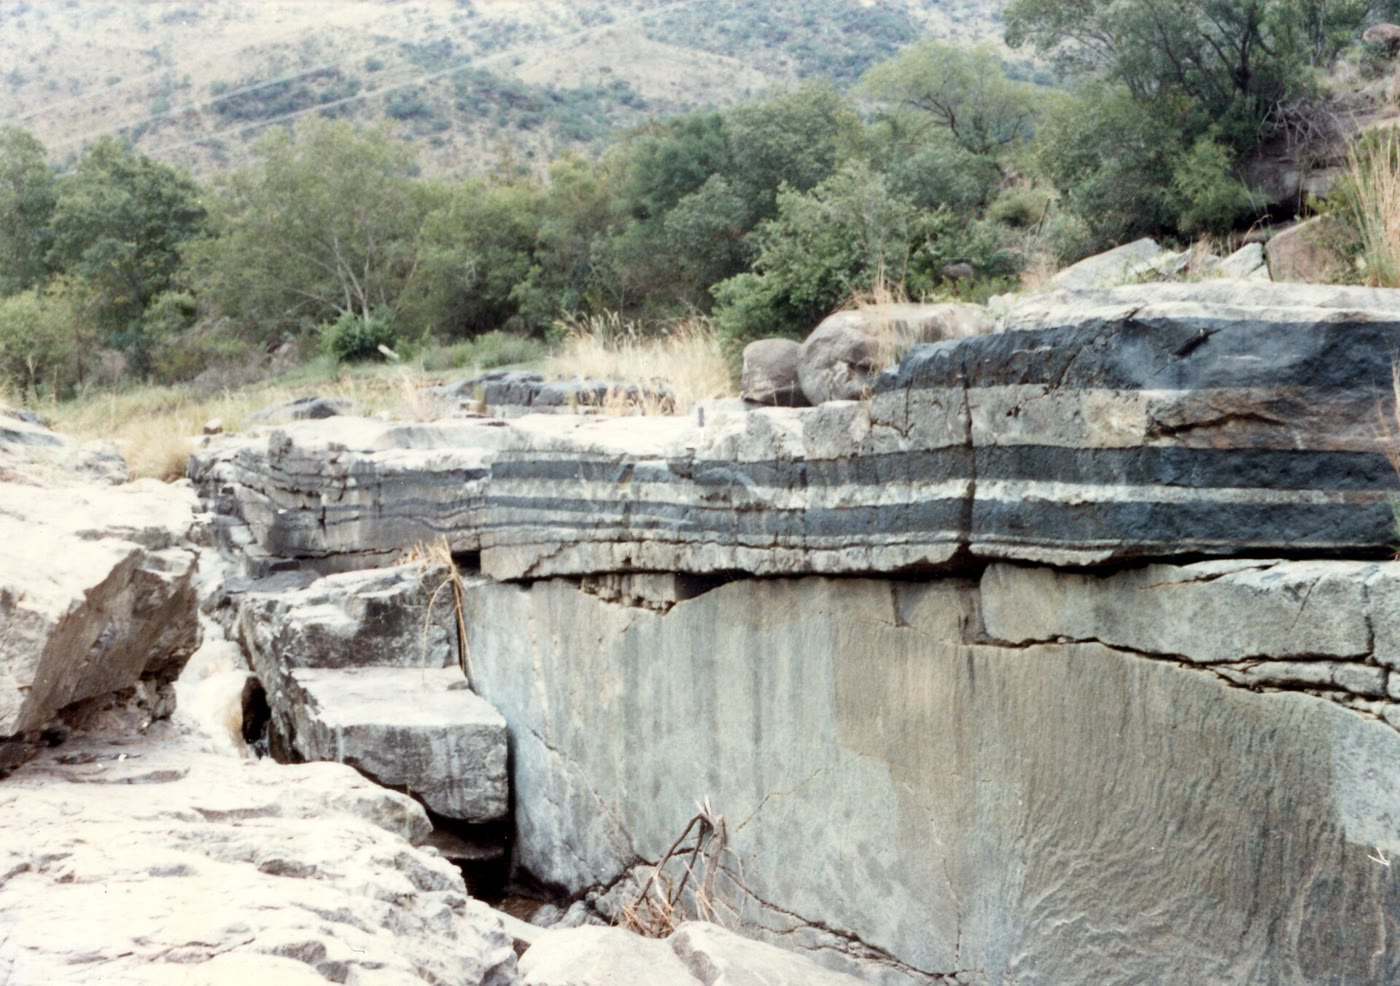
\includegraphics[height=5.2cm]{images/book4/b2-bushveld-chromitite.jpg}
\end{minipage}\hfill
\begin{minipage}[t]{0.42\linewidth}\vspace{0pt}\centering
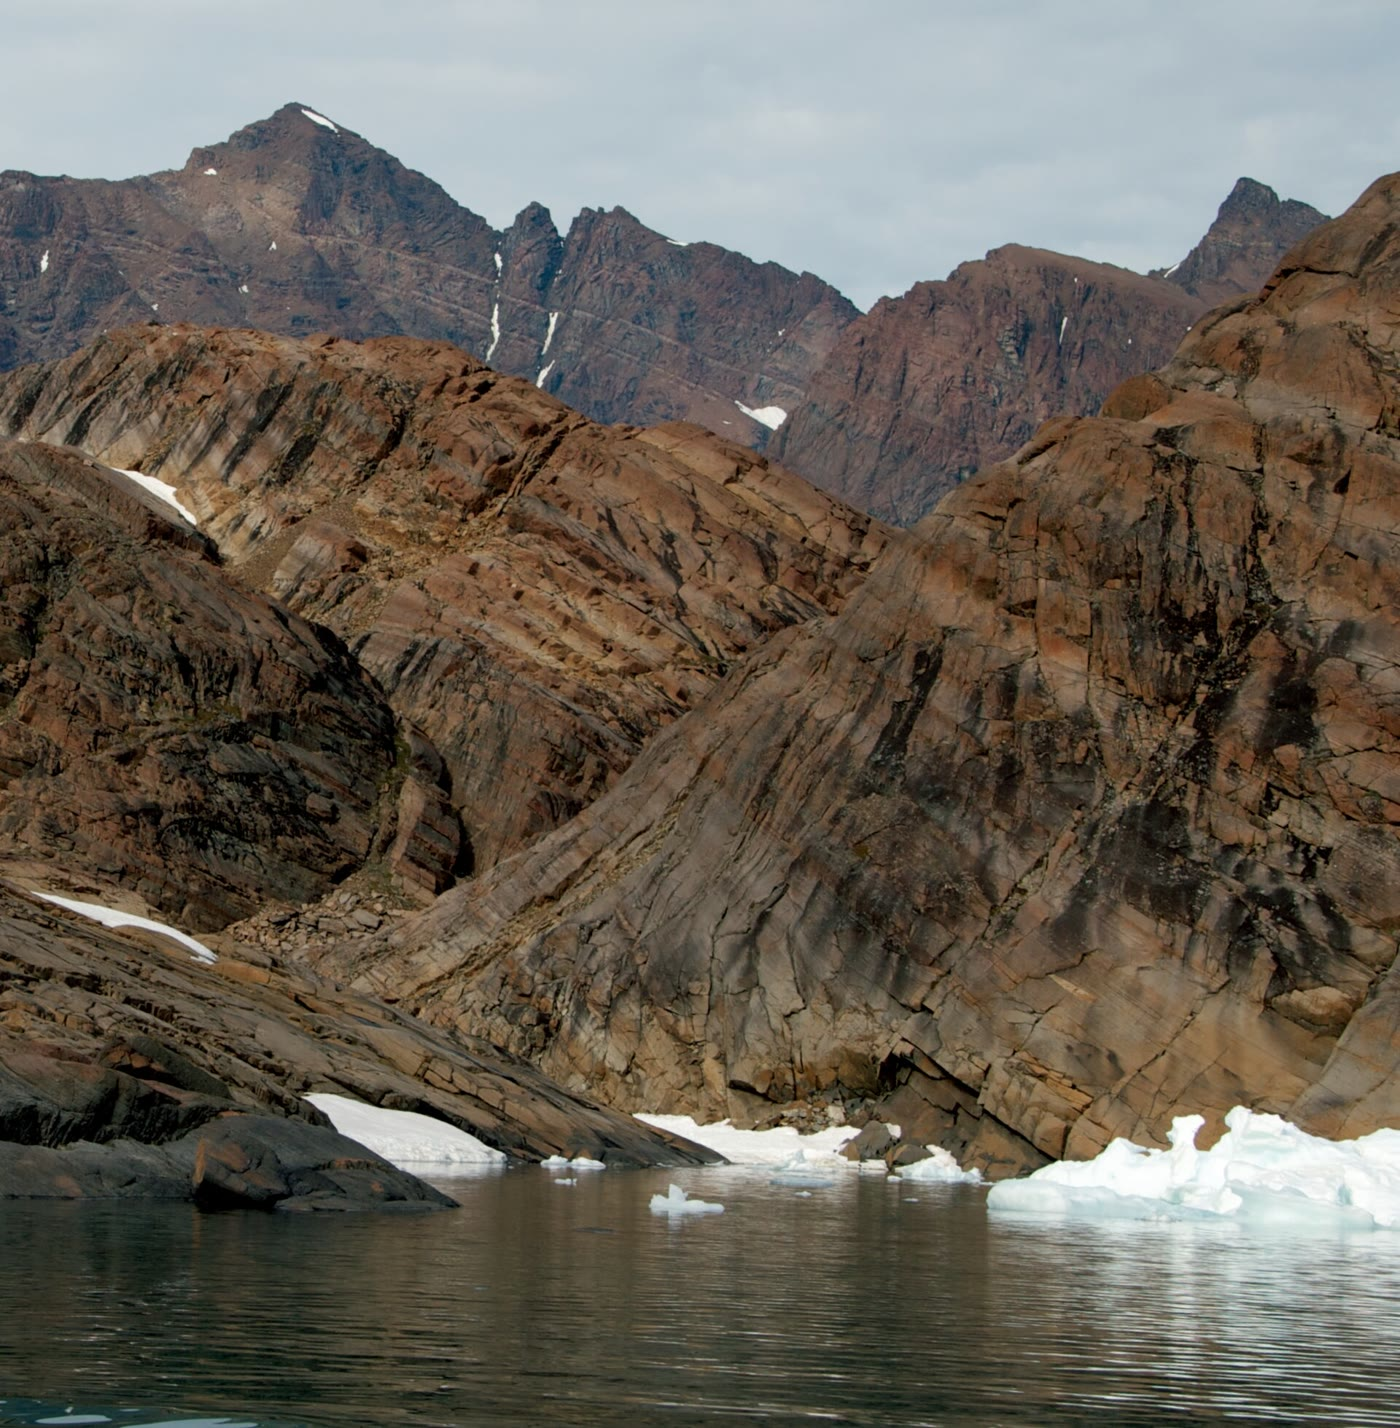
\includegraphics[height=5.2cm]{images/book4/b2-skaergaard-layering.jpg}
\end{minipage}
\par\smallskip{\small Links: zwarte lagen chromitiet en grijze lagen anorthosiet van de
Kritieke Zone van het Bushveldcomplex, Zuid-Afrika (Kevin Walsh, CC BY 2.0).
Rechts: de gelaagde gabbro's van de Middelste Zone van de Skaergaard-intrusie, Oost-Groenland,
hellend van linksboven naar rechtsonder (C. Tegner, CC BY 4.0).}
\end{omfigure}

\section{Open systemen}\label{sec:b2:magmatic-differentiation:open}

Een magmakamer is zelden gesloten. Nieuw \omterm{def:b2:magma-emplacement:magma}{magma} komt van onderen aan, en de wanden van de
kamer zijn gesteenten die het \omterm{def:b2:magma-emplacement:magma}{magma} kan verhitten, smelten en oplossen.

\begin{definition}[Magmamenging; korstassimilatie; AFC]
\label{def:b2:magmatic-differentiation:open}
\emph{Magmamenging}\index{magmamenging} is het samengaan van twee \omterm{def:b2:magma-emplacement:magma}{magma's} met verschillende
samenstellingen tot één. \emph{Korstassimilatie}\index{korstassimilatie} is de
opname van korstgesteente in een \omterm{def:b2:magma-emplacement:magma}{magma}, door smelten en oplossen van het
nevengesteente of van blokken die erin zijn gevallen.
\emph{Assimilatie--fractionele kristallisatie}\index{assimilatie--fractionele kristallisatie} (AFC) is hun
combinatie in één kamer: het \omterm{def:b2:magma-emplacement:magma}{magma} kristalliseert, en de vrijgekomen latente warmte
smelt en assimileert het nevengesteente.
\end{definition}

\begin{proposition}[Menging is lineair in de concentraties]\label{prop:b2:magmatic-differentiation:mixing}
Een mengsel van een massafractie $s$ \omterm{def:b2:magma-emplacement:magma}{magma} A en $1-s$ \omterm{def:b2:magma-emplacement:magma}{magma} B heeft voor elke
concentratie $C = sC_A + (1-s)C_B$: in elk diagram van de ene concentratie tegen
de andere liggen mengsels op het rechte lijnstuk van A naar B, en de hefboomregel geeft
$s$.
\end{proposition}

\begin{proof}
Elk element blijft behouden: $C(m_A + m_B) = m_AC_A + m_BC_B$; deel door $m_A + m_B$.
\end{proof}

Menging en het verwijderen van kristallen trekken beide rechte lijnen in \omterm{def:b2:magmatic-differentiation:harker}{Harkerdiagrammen};
isotopenverhoudingen onderscheiden ze. Kristallisatie verandert een isotopenverhouding niet, terwijl
menging met een gesteente met een andere verhouding dat wel doet, langs de hyperbool van
\cref{ch:b2:isotope-geochemistry}. Een stijging van $^{87}$Sr/$^{86}$Sr met silica in een
vulkanische reeks is daarom het kenmerk van assimilatie.

\begin{proposition}[Assimilatie met fractionele kristallisatie]
\label{prop:b2:magmatic-differentiation:afc}
Een \omterm{def:b2:magma-emplacement:magma}{magma} kristalliseert kristallen met globale verdelingscoëfficiënt $D$ voor een element
en assimileert nevengesteente met concentratie $C_a$ met een snelheid die $r$ keer de
kristallisatiesnelheid is ($r \ne 1$). Met $F$ de massa \omterm{def:b2:magma-emplacement:magma}{magma} ten opzichte van zijn
beginmassa en $z = (r + D - 1)/(r - 1)$ geldt
\[
\frac{C}{C_0} = F^{-z} + \frac{r}{r - 1 + D}\,\frac{C_a}{C_0}\,\bigl(1 - F^{-z}\bigr).
\]
Voor $r = 0$ is dit de wet van Rayleigh. De isotopenverhouding van het element in het \omterm{def:b2:magma-emplacement:magma}{magma}
is het gemiddelde van die van het beginmagma en die van het nevengesteente, gewogen met de
twee termen van deze som.
\end{proposition}

\begin{proof}
Per eenheid beginmassa wordt, wanneer een massa $\mathrm dm_c$ kristalliseert, een massa
$r\,\mathrm dm_c$ geassimileerd en verandert de magmamassa met $\mathrm dM =
-(1-r)\,\mathrm dm_c$. De balans van het element is $\mathrm d(MC) = rC_a\,\mathrm dm_c -
DC\,\mathrm dm_c$. Door het linkerlid uit te werken en $\mathrm dm_c$ te vervangen door
$-\mathrm dM/(1-r)$ volgt
\[
M\frac{\mathrm dC}{\mathrm dM} = -C - \frac{rC_a - DC}{1-r}
= \frac{(r - 1 + D)\,C - rC_a}{1 - r} = -z\,\bigl(C - C^*\bigr),
\qquad C^* = \frac{rC_a}{r - 1 + D}.
\]
Dus $\mathrm d(C - C^*)/(C - C^*) = -z\,\mathrm dM/M$, en $C - C^*$ is evenredig
met $M^{-z}$; met $C = C_0$ bij $M = 1$ volgt $C = C^* + (C_0 - C^*)F^{-z}$, wat de
formule is. Voor $r = 0$ geldt $z = 1 - D$ en $C^* = 0$. De atomen die uit het
beginmagma komen, gehoorzamen aan dezelfde vergelijking met $C_a = 0$, dus hun concentratie is
$C_0F^{-z}$; de rest komt uit de wand: vandaar de weging van de isotopenverhoudingen.
\end{proof}

DePaolo gaf deze vergelijkingen in 1981, en ze zijn het standaardmodel van een \omterm{def:b2:magma-emplacement:magma}{magma} dat
op zijn weg door de korst wordt verontreinigd. Ze verbergen een thermische voorwaarde. De warmte
om gesteente te assimileren komt van de latente warmte van de kristallen: korst verhitten van
150 tot \qty{1150}{\celsius} kost ongeveer \qty{1}{kJ/g}, haar smelten \qty{300}{J/g},
terwijl kristalliserend \omterm{def:b2:magma-emplacement:magma}{magma} ongeveer \qty{400}{J/g} levert; er moet dus zo'n \qty{3.25}{g}
\omterm{def:b2:magma-emplacement:magma}{magma} kristalliseren voor elke gram geassimileerd gesteente, en $r$ ligt ruim onder 1.
Wilcox maakte dezelfde berekening voor Parícutin: zijn \qty{25.4}{g}
kwartsmonzoniet, genomen bij ongeveer \qty{200}{\celsius}, had zo'n \qty{31350}{J} nodig om
tot \qty{1100}{\celsius} te worden verhit en gesmolten, de kristallisatiewarmte van ongeveer
\qty{85}{g} plagioklaas, veel meer dan de \qty{12.5}{g} kristallen die zijn
massabalans verwijderde. Het uitgebarsten \omterm{def:b2:magma-emplacement:magma}{magma} kon zijn eigen assimilatie niet hebben betaald:
de warmte moet zijn gekomen van een groter magmalichaam dan het lichaam dat uitbarstte,
dat buiten het zicht kristalliseerde (\cref{exo:b2:magmatic-differentiation:11}).
% ledger: depaolo81:afc, white09:afc-heat, wilcox54:heat, wilcox54:mass-balance

\begin{omfigure}
\centering
\begin{tikzpicture}
\begin{axis}[omrecord, name=left, width=0.47\linewidth, height=5.4cm,
  xmin=0.3, xmax=1, ymin=0.3, ymax=1.05, x dir=reverse,
  xlabel={overgebleven magma $F$}, ylabel={Sr: $C/C_0$},
  tick label style={font=\scriptsize}, label style={font=\small}]
\addplot[thick, black] table[x=F, y=srC_r0] {figdata/out/bachelor-2-differentiation-afc.dat};
\addplot[thick, blue!70!black] table[x=F, y=srC_r02] {figdata/out/bachelor-2-differentiation-afc.dat};
\addplot[thick, red!70!black] table[x=F, y=srC_r05] {figdata/out/bachelor-2-differentiation-afc.dat};
\end{axis}
\begin{axis}[omrecord, at={(left.east)}, anchor=west, xshift=1.7cm,
  width=0.47\linewidth, height=5.4cm,
  xmin=0.3, xmax=1, ymin=0.703, ymax=0.716, x dir=reverse,
  xlabel={overgebleven magma $F$}, ylabel={$^{87}$Sr/$^{86}$Sr},
  y tick label style={/pgf/number format/fixed, /pgf/number format/precision=3},
  legend style={font=\scriptsize, at={(0.03,0.97)}, anchor=north west},
  tick label style={font=\scriptsize}, label style={font=\small}]
\addplot[thick, black] table[x=F, y=iso_r0] {figdata/out/bachelor-2-differentiation-afc.dat};
\addlegendentry{$r = 0$}
\addplot[thick, blue!70!black] table[x=F, y=iso_r02] {figdata/out/bachelor-2-differentiation-afc.dat};
\addlegendentry{$r = 0.2$}
\addplot[thick, red!70!black] table[x=F, y=iso_r05] {figdata/out/bachelor-2-differentiation-afc.dat};
\addlegendentry{$r = 0.5$}
\end{axis}
\end{tikzpicture}
\par\smallskip{\small Assimilatie met \omterm{def:b2:magmatic-differentiation:crystallisation}{fractionele kristallisatie} voor strontium
($D = 1.5$, nevengesteente met de helft van het strontium van het \omterm{def:b2:magma-emplacement:magma}{magma} en
$^{87}$Sr/$^{86}$Sr = 0.7200, \omterm{def:b2:magma-emplacement:magma}{magma} 0.7035; illustratieve waarden). Links: de
concentratie daalt sneller naarmate de assimilatiesnelheid $r$ toeneemt, omdat het nevengesteente
minder strontium aanvoert en er voor dezelfde $F$ meer kristallen ontstaan. Rechts: de
isotopenverhouding, die door kristallisatie alleen niet verandert ($r = 0$), klimt naar die van de wand.}
\end{omfigure}

\section{Gezoneerde kristallen lezen}\label{sec:b2:magmatic-differentiation:zoning}

\begin{definition}[Samenstellingszonering]\label{def:b2:magmatic-differentiation:zoning}
Een kristal van een vaste oplossing vertoont \emph{samenstellingszonering}\index{samenstellingszonering}
wanneer zijn samenstelling van kern naar rand varieert, en zo de veranderende vloeistof vastlegt
waaruit de opeenvolgende lagen groeiden. De zonering is \emph{normaal} wanneer de rand rijker is aan
de lagetemperatuurcomponent (natrium in plagioklaas), \emph{omgekeerd} wanneer hij
rijker is aan de hogetemperatuurcomponent, en \emph{oscillerend} wanneer ze afwisselt.
\end{definition}

Een gezoneerd kristal is \omterm{def:b2:magmatic-differentiation:crystallisation}{fractionele kristallisatie} op heterdaad betrapt: zijn kern heeft zich
niet opnieuw met de latere vloeistof in evenwicht gesteld. De figuur hieronder berekent, op de lus van Bowen,
het plagioklaas dat groeit uit een vloeistof met \qty{50}{\percent} anorthiet. Bij
evenwicht blijven de kristallen homogeen en eindigen ze op \qty{50}{\percent}; bij volmaakte
\omterm{def:b2:magmatic-differentiation:crystallisation}{fractionele kristallisatie} is elke nieuwe laag in evenwicht met een steeds natriumrijkere
vloeistof, en is de rand van de laatste kristallen bijna zuiver albiet. Normale zonering, van
calciumrijke kern naar natriumrijke rand, is wat de reeks van Bowen voorspelt voor een afkoelend \omterm{def:b2:magma-emplacement:magma}{magma}. Een omgekeerde
zone, een calciumrijke band buiten een natriumrijke, zegt dat het kristal plotseling werd omspoeld door
een hetere of calciumrijkere vloeistof: vaak de aankomst van nieuw \omterm{def:b2:magma-emplacement:magma}{magma}, menging in de
kamer.
% ledger: bowen13:plagioclase, earle:bowen (Book 2)

\begin{omfigure}
\centering
\begin{tikzpicture}
\begin{axis}[omrecord, width=0.78\linewidth, height=6cm,
  xmin=0, xmax=1, ymin=0, ymax=90,
  xlabel={gekristalliseerde fractie van de vloeistof},
  ylabel={anorthiet (\unit{\percent}, moleculair)},
  legend style={font=\scriptsize, at={(0.02,0.02)}, anchor=south west},
  tick label style={font=\scriptsize}, label style={font=\small}]
\addplot[very thick, red!70!black] table[x=x, y=an_frac] {figdata/out/bachelor-2-differentiation-zoning.dat};
\addlegendentry{fractioneel: laag in vorming}
\addplot[thick, gray, densely dotted] table[x=x, y=an_liq_frac] {figdata/out/bachelor-2-differentiation-zoning.dat};
\addlegendentry{fractioneel: vloeistof}
\addplot[very thick, blue!70!black, dashed] table[x=x, y=an_eq] {figdata/out/bachelor-2-differentiation-zoning.dat};
\addlegendentry{evenwicht: kristallen}
\end{axis}
\end{tikzpicture}
\par\smallskip{\small Plagioklaas dat kristalliseert uit een vloeistof met \qty{50}{\percent}
anorthiet, berekend op de lus van Bowen (1913). Bij \omterm{def:b2:magmatic-differentiation:crystallisation}{fractionele kristallisatie} worden de
opeenvolgende lagen van de kristallen, van kern (links) naar rand (rechts), steeds
natriumrijker, en bereikt de vloeistof albiet wanneer ongeveer \qty{82}{\percent} is gekristalliseerd; bij
\omterm{def:b2:magmatic-differentiation:crystallisation}{evenwichtskristallisatie} blijven de kristallen uniform en eindigen ze met de samenstelling van
de vloeistof waaruit ze kwamen.}
\end{omfigure}

\begin{inthelab}[Gezoneerde kristallen lezen]
Petrologen lezen zonering eerst tussen gekruiste nicols, waar de zones van een
plagioklaas bij iets verschillende hoeken uitdoven en als concentrische banden verschijnen.
Daarna meten ze haar: een elektronenmicrosonde (\cref{ch:b2:field-lab-methods-2})
analyseert vlekjes van enkele micrometer langs een traverse van kern naar rand, en kaarten
van calcium en natrium tonen de zones rechtstreeks. Uit zo'n profiel berekenen ze de
samenstelling van de vloeistof waaruit elke zone groeide, met de lus van de figuur hierboven of
met verdelingscoëfficiënten, en ze tellen de omgekeerde zones als het aantal
aanvullingen van de kamer. \omterm{def:b2:elements-in-the-earth:trace}{Sporenelementen} die langs dezelfde traverse met
laserablatie worden gemeten, en isotopenverhoudingen die zone per zone worden gemeten, scheiden kristallisatie, menging
en assimilatie in de geschiedenis van één enkel kristal.
\end{inthelab}

\section{Oefeningen}

\begin{exercise}[$\star$]\label{exo:b2:magmatic-differentiation:1}
Gebruik de metingen van Bowen aan de plagioklazen (solidus / liquidus, \unit{\celsius}):
An$_{100}$ 1550 / 1550; An$_{83.3}$ 1465 / 1521; An$_{66.7}$ 1372 / 1490; An$_{50}$
1287 / 1450; An$_{33.3}$ 1205 / 1394; An$_{20}$ liquidus 1334; An$_{11.1}$ liquidus
1265, en interpoleer lineair tussen naburige punten. Een vloeistof met
\qty{50}{\percent} anorthiet koelt af in evenwicht. (a) Bepaal bij welke temperatuur ze
begint te kristalliseren, en de samenstelling van het eerste kristal. (b) Bepaal bij
\qty{1394}{\celsius} de samenstellingen van de vloeistof en van de kristallen,
en de gekristalliseerde massafractie (gebruik molfracties alsof het
massafracties waren). (c) Bepaal de samenstelling van de laatste druppel vloeistof.
\end{exercise}
% ledger: bowen13:plagioclase

\begin{exercise}[$\star$]\label{exo:b2:magmatic-differentiation:2}
Een gabbroïsch \omterm{def:b2:magmatic-differentiation:cumulate}{cumulaat} bevat \qty{50}{\percent} plagioklaas, \qty{35}{\percent}
clinopyroxeen en \qty{15}{\percent} olivijn. Bereken met de verdelingscoëfficiënten
(olivijn / clinopyroxeen / plagioklaas) Sr 0.000063 / 0.157 / 2.7, Zr 0.00068 /
0.195 / 0.001 en Rb 0.000044 / 0.0033 / 0.025 de globale
verdelingscoëfficiënt van elk element, en zeg welk compatibel is.
\end{exercise}
% ledger: white07:kd-basalt

\begin{exercise}[$\star$]\label{exo:b2:magmatic-differentiation:3}
Het \omterm{def:b2:magmatic-differentiation:cumulate}{cumulaat} van \cref{exo:b2:magmatic-differentiation:2} kristalliseert door \omterm{def:b2:magmatic-differentiation:crystallisation}{fractionele kristallisatie} uit een basalt,
tot de helft van de vloeistof over is. (a) Bepaal met welke factor Sr, Zr en Rb elk zijn veranderd
in de vloeistof (neem de globale coëfficiënten 1.40, 0.069 en 0.014). (b) Bepaal met welke factor
de verhouding Zr/Rb is veranderd. Becommentarieer aan de hand van het gevolg over verhoudingen.
\end{exercise}
% ledger: white07:kd-basalt

\begin{exercise}[$\star$]\label{exo:b2:magmatic-differentiation:4}
De eerste lava van Parícutin (februari 1943) had \qty{55.04}{\percent} \ce{SiO2},
\qty{5.68}{\percent} \ce{MgO} en \qty{0.85}{\percent} \ce{K2O}; de laatste (februari
1952), 60.07, 3.73 en \qty{1.67}{\percent}. (a) Bereken de verandering van elk oxide.
(b) Kali gaat in geen van de kristalliserende mineralen. Bepaal welke fractie van de vloeistof
over zou zijn geweest als het alleen door \omterm{def:b2:magmatic-differentiation:crystallisation}{fractionele kristallisatie} was geconcentreerd.
(c) De massabalans van Wilcox verwijdert maar ongeveer \qty{12.5}{g} kristallen per
\qty{100}{g} \omterm{def:b2:magma-emplacement:magma}{magma}. Wat suggereert de vergelijking?
\end{exercise}
% ledger: wilcox54:table2, wilcox54:mass-balance

\begin{exercise}[$\star\star$]\label{exo:b2:magmatic-differentiation:5}
Vergelijk \omterm{def:b2:magmatic-differentiation:crystallisation}{fractionele kristallisatie} en \omterm{def:b2:magmatic-differentiation:crystallisation}{evenwichtskristallisatie}: bereken $C_L/C_0$ met beide wetten
(a) voor nikkel, $D = 5$, wanneer \qty{20}{\percent} van de vloeistof is gekristalliseerd; (b)
voor een \omterm{def:b2:elements-in-the-earth:partition}{incompatibel element}, $D = 0.01$, wanneer \qty{90}{\percent} is gekristalliseerd.
(c) Bepaal de limieten van beide wetten voor $F \to 0$. Welke wet kan een vloeistof volledig van een
\omterm{def:b2:elements-in-the-earth:partition}{compatibel element} ontdoen?
\end{exercise}

\begin{exercise}[$\star\star$]\label{exo:b2:magmatic-differentiation:6}
(a) Bereken de massapercentages \ce{MgO}, \ce{FeO} en \ce{SiO2} in olivijn
Fo$_{80}$, $(\ce{Mg}_{0.8}\ce{Fe}_{0.2})_2\ce{SiO4}$ ($M$ = 40.30, 71.84 en
\qty{60.08}{g/mol}). (b) Een basalt met \qty{10.0}{\percent} \ce{MgO} en
\qty{49.0}{\percent} \ce{SiO2} kristalliseert alleen deze olivijn tot zijn vloeistof
\qty{8.0}{\percent} \ce{MgO} bevat. Bepaal welke massafractie olivijn werd verwijderd. (c) Bepaal
dan het silicagehalte van de vloeistof.
\end{exercise}

\begin{exercise}[$\star\star$]\label{exo:b2:magmatic-differentiation:7}
Voor de Skaergaard-intrusie geldt $F = \num{1.091e-7}H^2 - \num{5.9064e-4}H + 0.7678$.
(a) Bereken $F$ bij $H = 0$, 1000 en \qty{2000}{m}. (b) Bepaal op welke hoogte $F = 0$.
(c) Bepaal welke fractie van het \omterm{def:b2:magma-emplacement:magma}{magma} was gekristalliseerd voordat de basis van de dagzomende
bodemopeenvolging ontstond, en waar die zich zou kunnen bevinden.
\end{exercise}
% ledger: tegner23:skaergaard

\begin{exercise}[$\star\star$]\label{exo:b2:magmatic-differentiation:8}
Langs het profiel van Skaergaard bevat het mediane \omterm{def:b2:magmatic-differentiation:cumulate}{cumulaat} \qty{177}{ppm} Ni bij
$F = 0.70$ (Onderste Zone a), \qty{54}{ppm} bij $F = 0.29$ (Middelste Zone) en
\qty{6.2}{ppm} bij $F = 0.17$ (Bovenste Zone a). (a) Neem aan dat de \omterm{def:b2:magmatic-differentiation:cumulate}{cumulaten}
$D$ keer het nikkel van hun vloeistof bevatten en dat de vloeistof de wet van Rayleigh volgt, en
bereken de schijnbare $D$ tussen de eerste twee niveaus. (b) Doe hetzelfde tussen de
laatste twee. (c) Wat kan de schijnbare $D$ doen veranderen?
\end{exercise}
% ledger: data:b4-skaergaard

\begin{exercise}[$\star\star$]\label{exo:b2:magmatic-differentiation:9}
Controleer het antwoord van Wilcox: \qty{100}{g} grondmassa van de eerste lava (\ce{SiO2}
55.53, \ce{MgO} 4.66, \ce{K2O} \qty{0.88}{\percent}) plus \qty{25.4}{g} gemiddelde
xenoliet (72.48, 0.77, 3.64) min \qty{2.9}{g} olivijn Fo$_{80}$ (39.19, 42.06, 0)
min \qty{9.6}{g} plagioklaas An$_{70}$ (50.54, 0, 0). (a) Bepaal welke massa overblijft.
(b) Bereken het \ce{SiO2}, \ce{MgO} en \ce{K2O} ervan en vergelijk met de grondmassa van
lava 19 (60.16, 3.19 en \qty{1.75}{\percent}). (c) Welk oxide past het slechtst?
\end{exercise}
% ledger: wilcox54:groundmass, wilcox54:xenoliths, wilcox54:mass-balance

\begin{exercise}[$\star\star\star$]\label{exo:b2:magmatic-differentiation:10}
Een \omterm{def:b2:magma-emplacement:magma}{magma} assimileert nevengesteente met $r = 0.2$ terwijl het kristalliseert, met $D_{\ce{Sr}} =
1.5$, $C_a/C_0 = 0.5$, begin-$^{87}$Sr/$^{86}$Sr = 0.7035 en nevengesteente 0.7200.
(a) Bereken $z$, $F^{-z}$ en $C/C_0$ bij $F = 0.7$. (b) Vergelijk met zuivere \omterm{def:b2:magmatic-differentiation:crystallisation}{fractionele
kristallisatie} bij dezelfde $F$, en verklaar het verschil met de massa kristallen
die in elk geval ontstaat. (c) Bereken de $^{87}$Sr/$^{86}$Sr van het \omterm{def:b2:magma-emplacement:magma}{magma}.
\end{exercise}

\begin{exercise}[$\star\star\star$]\label{exo:b2:magmatic-differentiation:11}
Volg het warmtebudget van Wilcox voor Parícutin. (a) Bepaal hoeveel warmte een gram
kwartsmonzoniet nodig heeft om van 200 tot \qty{1100}{\celsius} te gaan (warmtecapaciteit
\qty{1.1}{J/(g.K)}) en daarna te smelten (\qty{250}{J/g}). (b) Bepaal hoeveel voor
\qty{25.4}{g}. (c) Bepaal welke massa plagioklaas An$_{70}$ (latente warmte \qty{370}{J/g})
moet kristalliseren om haar te leveren. (d) Vergelijk met de \qty{12.5}{g} kristallen van de
massabalans, bereken de verhouding $r$ van assimilatie tot kristallisatie, en zeg wat
dit inhoudt.
\end{exercise}
% ledger: wilcox54:heat, white09:afc-heat

\begin{exercise}[$\star\star\star$]\label{exo:b2:magmatic-differentiation:12}
Een basalt met \qty{250}{ppm} Ni kristalliseert eerst alleen olivijn ($D = 5$) tot
$F = 0.8$, daarna olivijn met plagioklaas en clinopyroxeen (globale $D = 1.5$). (a)
Bereken de factor waarmee nikkel in elke etappe verandert, en het nikkelgehalte van
de vloeistof bij $F = 0.5$. (b) Bepaal wat één enkele wet met $D = 5$ zou hebben voorspeld.
(c) Verklaar waarom de wet van Rayleigh in etappes moet worden toegepast.
\end{exercise}

\section{Probleem: De intrusie die haar eigen geschiedenis schreef}

\begin{problem}[{Weekendprobleem --- van de lagen van een gabbro naar de fractie van
zijn magma die aan het eind nog vloeibaar was}]
\label{pb:b2:magmatic-differentiation:1}
Een (verzonnen) gelaagde gabbrosill kristalliseerde uit een basalt waarvan de \omterm{def:b2:magma-emplacement:aureole}{afschrikrand}
de oudersamenstelling geeft: \ce{SiO2} 49.5, \ce{Al2O3} 16.0, \ce{FeO} 10.0,
\ce{MgO} 9.0, \ce{CaO} 11.5, \ce{Na2O} 2.5, \ce{K2O} \qty{0.30}{\percent};
\qty{150}{ppm} Ni en \qty{80}{ppm} Zr. De \omterm{def:b2:magmatic-differentiation:cumulate}{cumulaten} van de onderste zone bestaan uit
\qty{20}{\percent} olivijn, \qty{50}{\percent} plagioklaas en \qty{30}{\percent}
clinopyroxeen; boven het niveau waar olivijn verdwijnt, uit \qty{55}{\percent}
plagioklaas en \qty{45}{\percent} clinopyroxeen. Neem de verdelingscoëfficiënten
(olivijn / plagioklaas / clinopyroxeen) Ni 5.0 / 0 / 2.0 en Zr 0.0007 / 0.001 /
0.195. Samenstellingen van de mineralen (\unit{\percent}): olivijn \ce{MgO} 42.06, \ce{CaO} 0,
\ce{Al2O3} 0, \ce{SiO2} 39.19; plagioklaas 0, 14.36, 31.70, 50.54; clinopyroxeen
16.0, 20.5, 3.0, 51.5. Een \omterm{def:b2:magma-emplacement:bodies}{gang}
van fijnkorrelig gesteente, gevoed vanuit de kamer toen de bovenste laag kristalliseerde, heeft
\ce{SiO2} 50.0, \ce{Al2O3} 14.1, \ce{FeO} 16.7, \ce{MgO} 4.9, \ce{CaO} 7.3,
\ce{Na2O} 3.4, \ce{K2O} \qty{0.75}{\percent} en \qty{188}{ppm} Zr.

\noindent\textbf{Deel I --- De verdelingscoëfficiënten van de lagen.}
\begin{enumerate}
\item Bereken de globale verdelingscoëfficiënt van nikkel in de onderste zone.
\item Bereken die van zirkonium in de onderste zone.
\item Bereken beide in de bovenste zone.
\item Zeg welk element in elke zone compatibel is. Blijft nikkel compatibel wanneer
olivijn verdwijnt?
\item Zeg welk mineraal het meeste zirkonium van de \omterm{def:b2:magmatic-differentiation:cumulate}{cumulaten} bevat, en waarom.
\item Bepaal met welke factor Ni/Zr in de vloeistof verandert per halvering van $F$ in de onderste
zone.
\end{enumerate}

\noindent\textbf{Deel II --- Rayleighkrommen langs het profiel omhoog.}
\begin{enumerate}[resume]
\item Bepaal welk nikkelgehalte te verwachten is in het onderste \omterm{def:b2:magmatic-differentiation:cumulate}{cumulaat}, gekristalliseerd bij
$F = 1$.
\item Een \omterm{def:b2:magmatic-differentiation:cumulate}{cumulaat} van de onderste zone hoger in het profiel bevat \qty{190}{ppm} Ni. Bepaal bij welke $F$ het
ontstond.
\item Bepaal het zirkoniumgehalte van de vloeistof op dat moment.
\item Vergelijk bij die $F$ het nikkel van de vloeistof volgens de fractionele en de
evenwichtswet.
\item Olivijn verdwijnt bij $F = 0.55$. Bereken het nikkelgehalte van de vloeistof
op dat punt.
\item Bereken het nikkel van de \omterm{def:b2:magmatic-differentiation:cumulate}{cumulaten} die net onder en net boven dat
niveau ontstaan. Welk kenmerk zou een geoloog in het profiel zien?
\item Bereken het nikkel van de vloeistof en van het \omterm{def:b2:magmatic-differentiation:cumulate}{cumulaat} bij $F = 0.40$. Verklaar
de trend.
\end{enumerate}

\noindent\textbf{Deel III --- De massabalans van de laatste vloeistof.}
\begin{enumerate}[resume]
\item Schrijf de behoudsvergelijking van de methode voor één oxide, met de massa's
$x_{\mathrm{ol}}, x_{\mathrm{pl}}, x_{\mathrm{cpx}}$ die per \qty{100}{g}
ouder worden verwijderd en de \omterm{def:b2:magma-emplacement:bodies}{gang} als dochter.
\item Schrijf ze voor \ce{MgO}, \ce{CaO} en \ce{Al2O3}.
\item Los het $3 \times 3$-stelsel op.
\item Bepaal welke fractie van de ouder als vloeistof overblijft.
\item Controleer het antwoord met \ce{SiO2}: bereken het silica van de vloeistof opnieuw uit de
gevonden massa's.
\item Vergelijk de verhoudingen van de verwijderde mineralen met de modi van de twee
zones.
\item Kali gaat in geen van de mineralen: bepaal welke fractie vloeistof het geeft.
\end{enumerate}

\noindent\textbf{Deel IV --- De fractie vloeistof aan de top.}
\begin{enumerate}[resume]
\item Bepaal met welke factor zirkonium in de vloeistof was gestegen toen olivijn verdween bij
$F = 0.55$. Geef het zirkoniumgehalte op dat moment.
\item Bereken uit het zirkonium van de \omterm{def:b2:magma-emplacement:bodies}{gang} de fractie vloeistof die over was toen
die ontstond, door de wet van de bovenste zone toe te passen vanaf $F = 0.55$.
\item Herhaal de berekening met één enkele $D = 0.07$ vanaf het begin. Is het antwoord
gevoelig voor de details van $D$?
\item IJzer steeg in de vloeistof van 10.0 tot \qty{16.7}{\percent}, terwijl silica nauwelijks
veranderde. Zeg welke mineralen daarvoor verantwoordelijk zijn, en welk soort magmatische reeks
dit aankondigt (\cref{ch:b2:magmatic-series}).
\item De bovenste \omterm{def:b2:magmatic-differentiation:cumulate}{cumulaten} bevatten \qty{47}{ppm} Zr. Cumuluskristallen alleen zouden
$\bar D$ keer het zirkonium van de vloeistof bevatten; bepaal welke massafractie gevangen vloeistof
(met de samenstelling van de \omterm{def:b2:magma-emplacement:bodies}{gang}) de analyse verklaart.
\item Geef de fractie van het oorspronkelijke \omterm{def:b2:magma-emplacement:magma}{magma} die nog vloeibaar was toen de bovenste laag
kristalliseerde, het kerngetal van dit probleem, en vergelijk de drie schattingen
(hoofdelementen, kali, zirkonium).
\end{enumerate}
\end{problem}
% ledger: white07:kd-basalt, matzen12:dni
